% Scatter plot using TikZ and pgfplots
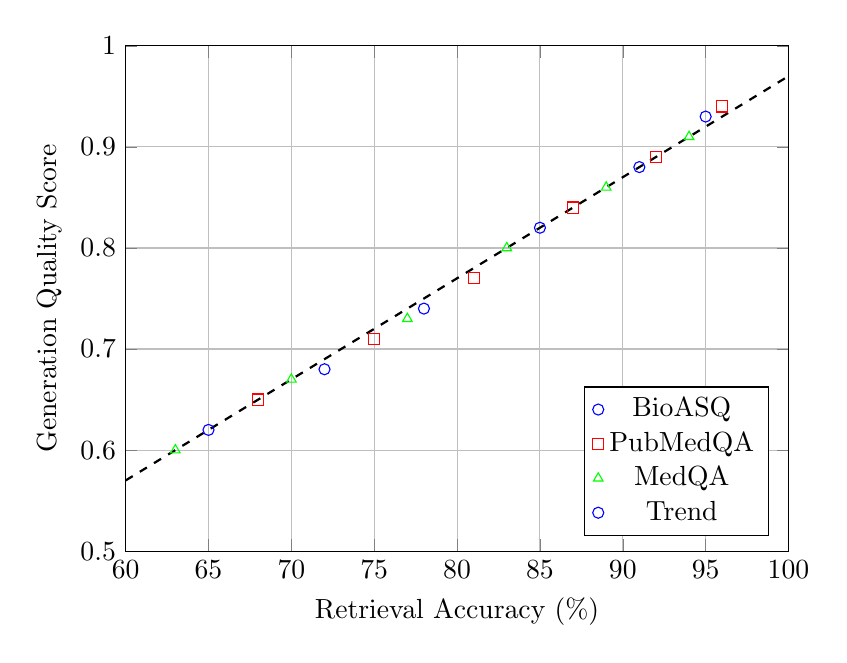
\begin{tikzpicture}
\begin{axis}[
    width=10cm,
    height=8cm,
    xlabel={Retrieval Accuracy (\%)},
    ylabel={Generation Quality Score},
    xmin=60, xmax=100,
    ymin=0.5, ymax=1.0,
    grid=major,
    legend pos=south east,
    scatter/classes={
        a={mark=o,draw=blue,fill=blue!20},
        b={mark=square,draw=red,fill=red!20},
        c={mark=triangle,draw=green,fill=green!20}
    }
]

% Dataset 1
\addplot[scatter,only marks,scatter src=explicit symbolic]
coordinates {
    (65,0.62) [a]
    (72,0.68) [a]
    (78,0.74) [a]
    (85,0.82) [a]
    (91,0.88) [a]
    (95,0.93) [a]
};
\addlegendentry{BioASQ}

% Dataset 2
\addplot[scatter,only marks,scatter src=explicit symbolic]
coordinates {
    (68,0.65) [b]
    (75,0.71) [b]
    (81,0.77) [b]
    (87,0.84) [b]
    (92,0.89) [b]
    (96,0.94) [b]
};
\addlegendentry{PubMedQA}

% Dataset 3
\addplot[scatter,only marks,scatter src=explicit symbolic]
coordinates {
    (63,0.60) [c]
    (70,0.67) [c]
    (77,0.73) [c]
    (83,0.80) [c]
    (89,0.86) [c]
    (94,0.91) [c]
};
\addlegendentry{MedQA}

% Trend line
\addplot[domain=60:100,samples=2,dashed,thick,black]{0.01*x - 0.03};
\addlegendentry{Trend}

\end{axis}
\end{tikzpicture}
